\documentclass{article}
\linespread{1.5}

\usepackage[utf8]{inputenc}
\usepackage{natbib}
\usepackage{graphicx}
\usepackage{authblk}
%For line number
\usepackage{lineno}

\title{Supplementary Information\\ Playing the political game: The co-evolution of institutions with group size and political inequality}


\author[1]{Simon T.Powers}
\author[2]{Cedric Perret}
\author[2]{Thomas E. Currie}

\affil[1]{Edinburgh Napier University, Edinburgh EH10 5DT}
\affil[2]{University of Exeter, Penryn TR10 9Fr}
\date{In: Philosophical transactions of the Royal Society B\\
DOI: }


\begin{document}

\maketitle  

\begin{figure}, 
    \centering
    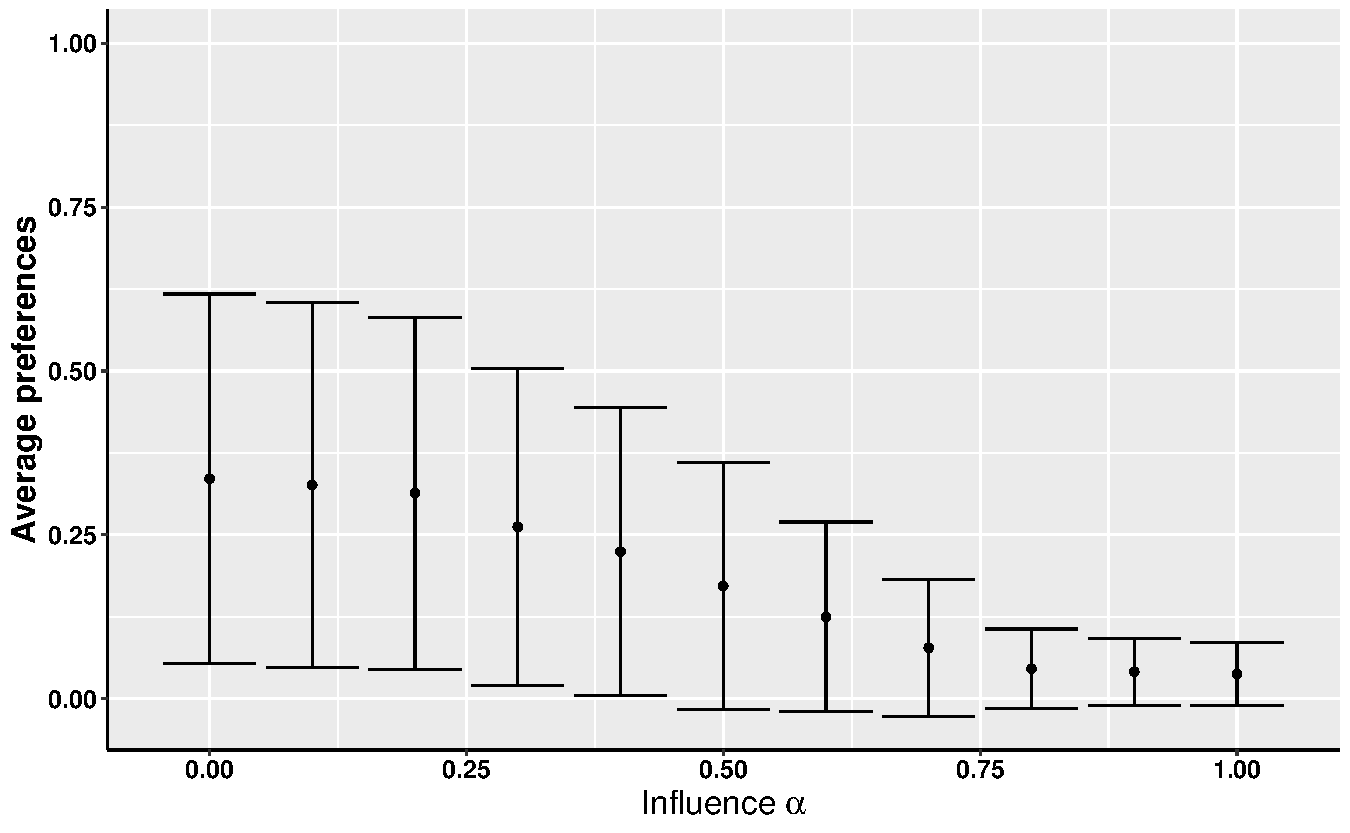
\includegraphics[width=1.2\linewidth]{Figures/pt_p_alpha.pdf}
    \caption{Average preferences as a function of influence, $\alpha$. The results presented are after 25 000 generations to avoid the effect of initial conditions. Error bars show the standard deviation}
    \label{figalpha}
\end{figure}


\begin{figure}, 
    \centering
    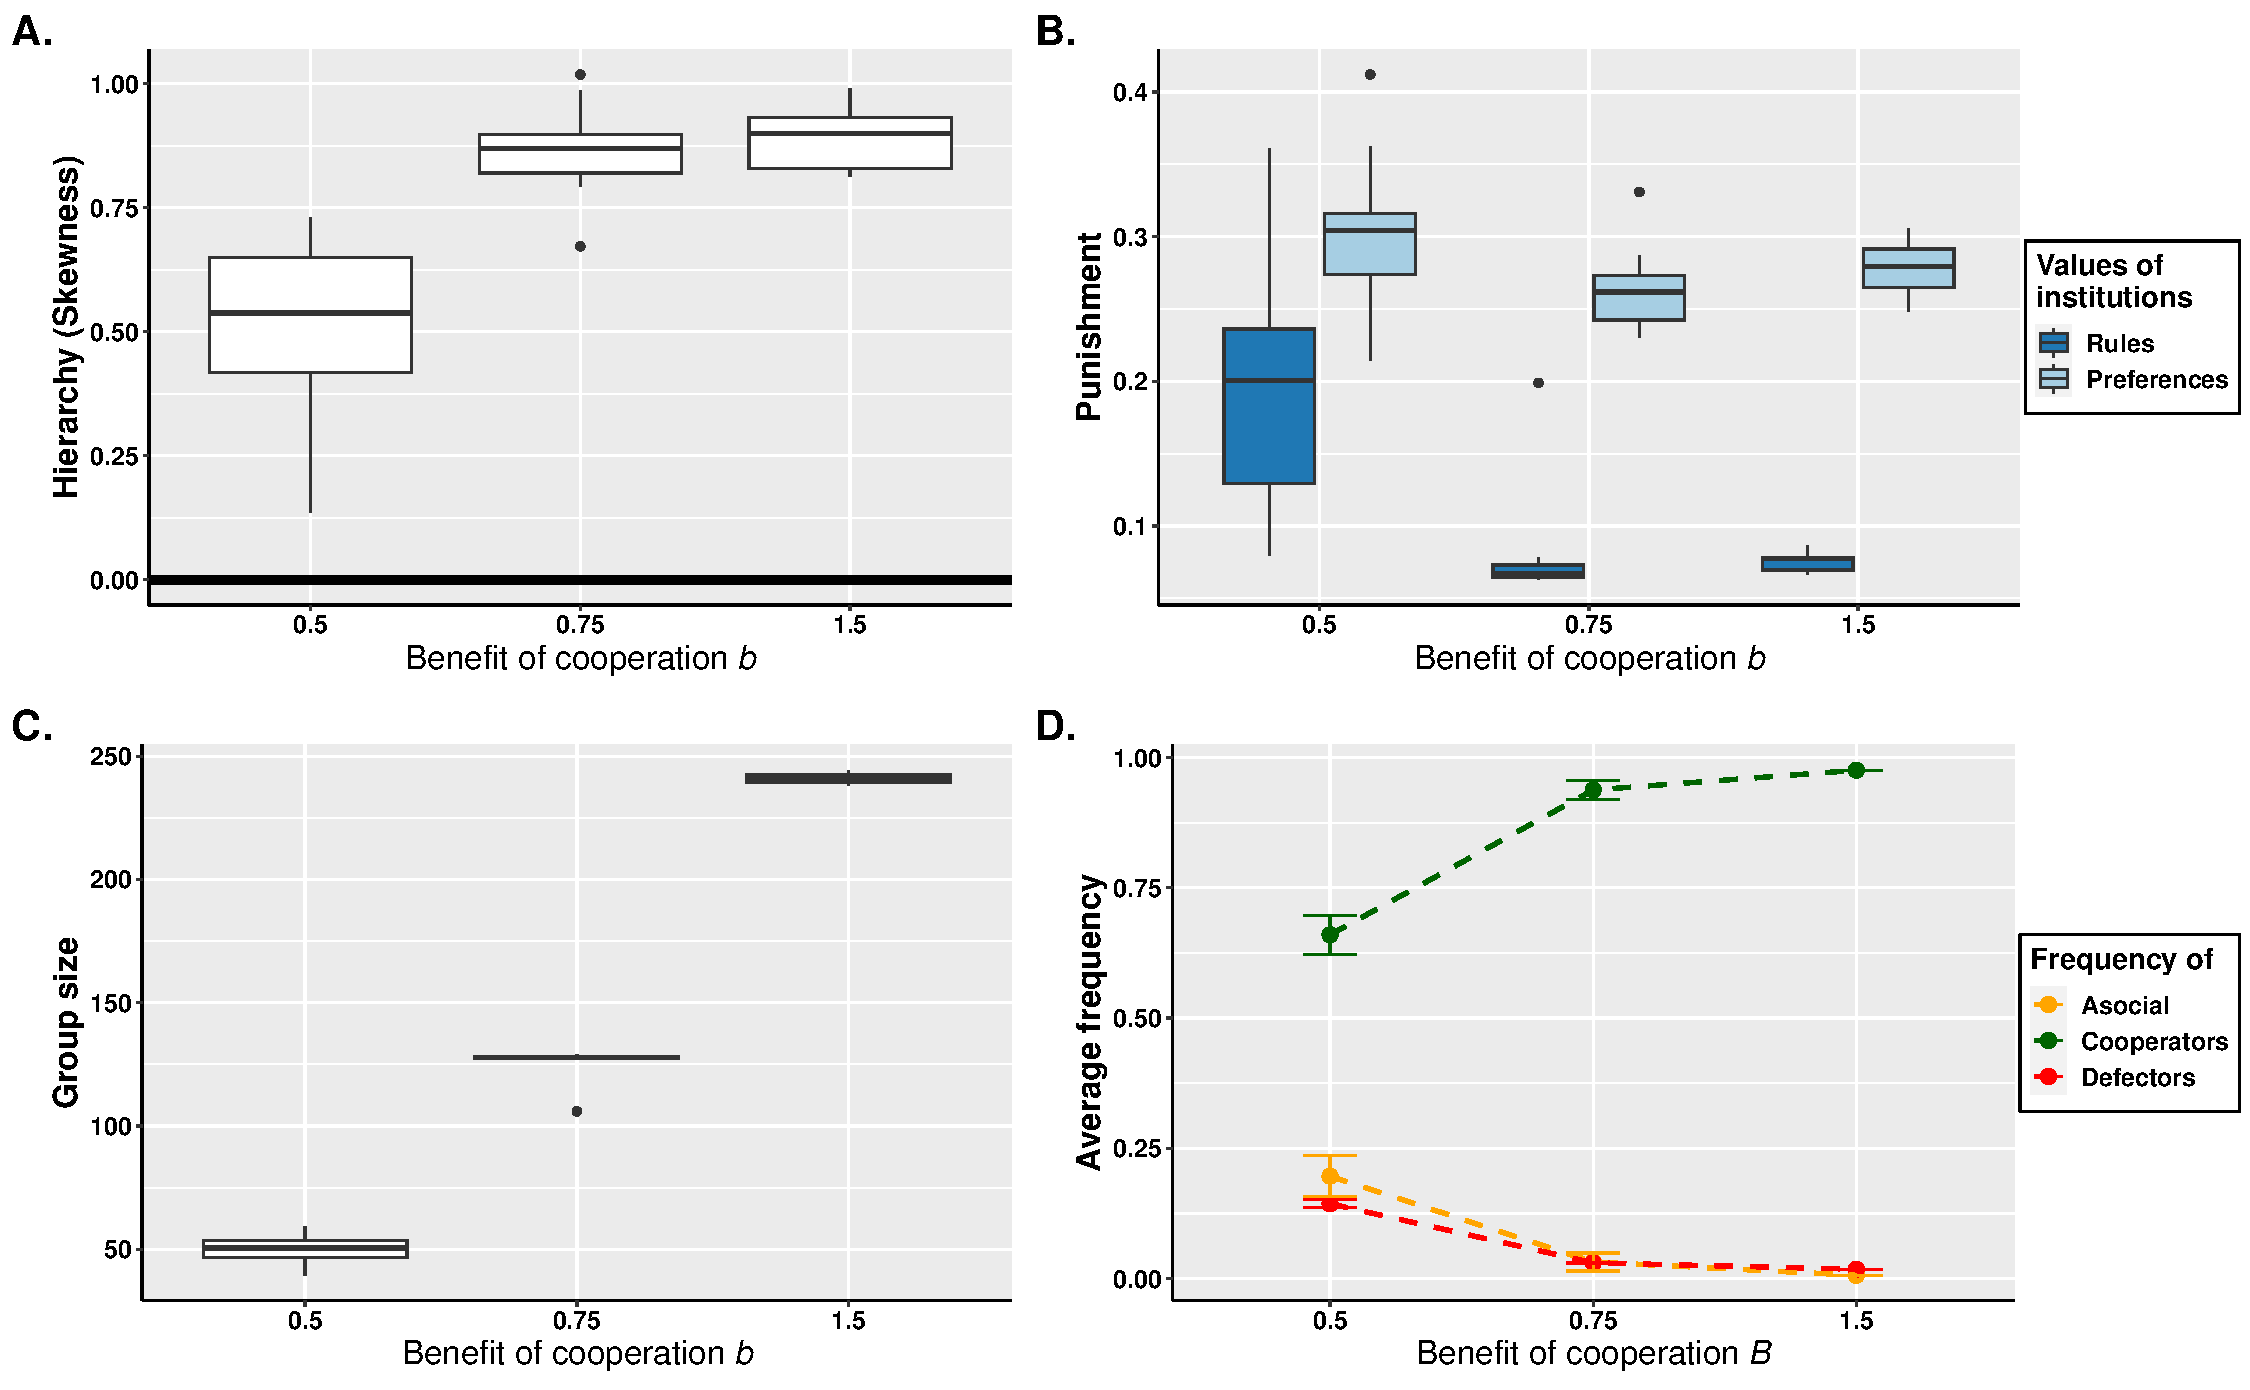
\includegraphics[width=1.2\linewidth]{Figures/pt_coopB.pdf}
    \caption{The effect of varying the benefit of cooperation $B$ on (A.) hierarchy, (B.) institutional rules and preferences, (C.) group size and (D.) frequency of each strategy. The boxplots represent measures across 50 000 generations and 10 replicates. Error bars in plot (D.) represent the standaerd deviation.}
    \label{figcoopB}
\end{figure}



\end{document}